\documentclass[UTF8]{beamer}
\usepackage{graphicx, color}
\usepackage{algorithm2e}
\usepackage{zhspacing}
\usepackage{amsmath}

\usepackage{setspace}
\usepackage{listings}

\usepackage{tikz}
\usepackage{tikz-uml}

\lstset{language=C++}

\usepackage{underscore}
\usetheme{JuanLesPins}
\usepackage{fontspec}
\setsansfont{Microsoft YaHei}

\usepackage{enumerate}

\AtBeginSection[]{
  \frame{
    \frametitle{Next}
    \tableofcontents[currentsection, subsectionstyle=show/shaded/hide]
  }
}

\AtBeginSubsection[]{
  \frame{
    \frametitle{Next}
    \tableofcontents[currentsubsection]
  }
}

\title{Java in Bioinformatics}

\author{Gang Chen\\ chengang@bgitechsolutions.com}

\logo{\includegraphics[width=1.3cm]{bgi-logo.png}\includegraphics[width=2.5cm]{cuhklogo.png}}
\date{\today}




\begin{document}

\begin{frame}
\titlepage
\end{frame}

\begin{frame}[t]\frametitle{Outline}
\tableofcontents[hideallsubsections]
\end{frame}



\section{Object Oriented Programming in Java}

\subsection{Basic Ideas}
\begin{frame}
  \frametitle{Object-oriented Programming (OOP)}

  \begin{itemize}
  \item OO is a language-indedependent concept
  \item in principle not limited to programming (OO design)\\
    $\implies$ databases, business plans
  \item improves reusability and exchangability of code
  \item separation of partial problems
  \item ``real world'' modelling
  \item representation in \alert{Universal Markup Language} (UML)
  \end{itemize}
\end{frame}

\begin{frame}
  \frametitle{Object-oriented Programming (OOP)}
  \tikzumlset{font=\tiny}
  \begin{tikzpicture}[scale=1.1]
    \begin{umlsystem}[x=4, fill=red!10]{Introduction to Programming}
      \umlusecase{Lectures}
      \umlusecase[x=4]{Sections}

      \umlusecase[y=-1]{Assignments}
      \umlusecase[x=4, y=-1]{Fibonacci Sequence}
      \umlusecase[x=3, y=-1.7]{Language-sepcific}
    \end{umlsystem}

    \umlactor[scale=0.5]{Gang Chen}
    \umlactor[scale=0.5,y=-1.5]{Students}

    \umlassoc{Students}{usecase-1}
    \umlassoc{Gang Chen}{usecase-1}
    \umlassoc{Students}{usecase-3}
    \umlassoc{Gang Chen}{usecase-3}
    \umlinclude{usecase-1}{usecase-2}
    \umlinclude{usecase-3}{usecase-4}
    \umlinclude{usecase-3}{usecase-5}
  \end{tikzpicture}
\end{frame}

\begin{frame}
  \frametitle{Basic ideas}

  \begin{itemize}
  \item \alert{Everything is an object}\\
    \emph{Gang, students, lecture}\\
    \emph{project, world, spy, information}
  \item \alert{Objects interact by sending/receiving messages}\\
    \emph{Gang $\rightarrow$ students: object orientation is a concept}\\
    \emph{world $\rightarrow$ map: what is the object at
      position X?}\\
  \item \alert{An object consists of objects}\\
    \emph{a course consists of lectures}\\
    \emph{a world consists of land or water fields}\\
  \end{itemize}
\end{frame}


\begin{frame}
  \frametitle{Basic ideas}
  \begin{itemize}
  \item \alert{Every object has a type}\\
    \emph{Gang is a teacher}\\
    \emph{the map is a rectangle of land / water fields}
  \item \alert{All objects of the same type understand the same messages}\\
    \emph{all students hear the lecture}\\
    \emph{all spies can retrieve information}
  \end{itemize}
\end{frame}


\subsection{Concepts}
\begin{frame}[t]{Classes, Interfaces and Methodse}
    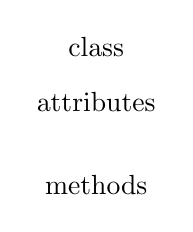
\begin{tikzpicture}[x=\textwidth,y=1em]
      \umlclass[x=0, y=0,type=abstract]{World}{
        spies : ListOfSpies
      }{
        setSpyCount(count: int)\\
        getSpyCount() : int\\[\smallskipamount]
    getMap() : Map
      }
      \draw (0.3, 3) node {\alert{class}};
      \draw (0.3, 1) node {\alert{attributes}};
      \draw (0.3, -2) node {\alert{methods}};

      \umlclass[x=0.6, y=0,type=abstract]{Map}{
        tiles: VectorOfTiles
      }{
        getWidth() : int\phantom{p}\\
        getHeight() : int\\[\smallskipamount]
        at(x: int, y:int) : Tile
      }

    \end{tikzpicture}
\end{frame}
%--- Next Frame ---%

\begin{frame}
  \frametitle{Classes, Interfaces and Methods}

  \begin{itemize}
    \item \alert{classes} describe the type of objects (define their \alert{interface})
    \item the interface consists of \alert{methods} and \alert{attributes} / properties
    \item methods
      \begin{itemize}
      \item are functions that operate on objects of this class
      \item can take extra arguments of arbitrary types
      \item can return values of arbitrary types
      \end{itemize}
    \item attributes are objects of arbitrary other types
  \end{itemize}
\end{frame}

\begin{frame}
  \frametitle{Objects/Instances}

  \begin{center}
    \begin{tikzpicture}[x=\textwidth]
      \begin{umlseqdiag}
      \umlobject[x=0.2,class=Map]{map}
      \umlobject[x=0.4,class=World]{world}
      \begin{umlcall}[op=width(),return=1234]{world}{map}\end{umlcall}
      \umlcreatecall[x=0.7,class={HQ},stereo=multi]{world}{headquarters}
      \umlcreatecall[x=0.7,class={Spy},stereo=multi]{world}{spy}
      \end{umlseqdiag}
    \end{tikzpicture}
  \end{center}

  \begin{itemize}
    \item every object has an immutable class assigned when it is created
    \item objects communicate via their class interfaces
    \item classes can communicate  via static member functions
  \end{itemize}
\end{frame}


\begin{frame}
  \frametitle{Overloading and signature}

  \begin{center}
    \begin{tikzpicture}
      \umlclass[type=abstract]{Spy}{ }{
        \umlvirt{setPos(x : int, y : int)}\\
        \umlvirt{setPos(pos: Position)}
      }
    \end{tikzpicture}
  \end{center}

  \begin{itemize}
  \item a method is described by name and \alert{signature}
  \item signature is formed by the types of all taken arguments
    \begin{itemize}
    \item setPos(\emph{x : int, y : int})\\
    \item setPos(\emph{pos : Position})
    \end{itemize}
  \item methods with identical names but different arguments can exist in one class -- \alert{overloading}
  \item return type is \emph{not} part of the signature -- cannot always resolve overload at compile time

  \end{itemize}
\end{frame}


\begin{frame}
    \frametitle{Composing classes}

  \begin{center}
    \begin{tikzpicture}
      \umlclass[type=abstract]{World}{
        map : Map
      }{
        setSpyCount(count : int)\\
        getSpyCount() : int
      }

      \umlclass[x=6,type=abstract]{Spy}{
        x, y : int
      }{
        \umlvirt{setPos(x : int, y : int)}\\
        \umlvirt{setPos(pos : Position)}
      }
      \umlunicompo[mult2=*,anchors=10 and 170]{World}{Spy}
      \umluniassoc[mult2=1,anchors=-170 and -10]{Spy}{World}
    \end{tikzpicture}
  \end{center}

    \begin{itemize}
    \item objects are made of objects (\alert{attributes}) ---\\
      classes declare the types of these objects
    \item simple attributes appear below class name
    \item complex classes shown as \alert{composition}
    \item ``has-a'' or ``has-many'' relations:
      \begin{itemize}
        \item \emph{a world hosts many spies},
        \item \emph{a spy belongs to one world}
      \end{itemize}
    \end{itemize}

\end{frame}

\begin{frame}
  \frametitle{Inheritance and class hierarchy}

  \begin{center}
    \begin{tikzpicture}
      \umlclass[y=1,x=4,type=abstract]{Tile}{
        map : Map
      }{
        \umlvirt{tryStep(...)}
      }
      \umlclass{WaterTile}{
      }{
        tryStep(...)
      }

      \umlclass[x=8]{LandTile}{
      }{
        tryStep(...)
      }

      \umlinherit{WaterTile}{Tile}
      \umlinherit{LandTile}{Tile}
    \end{tikzpicture}
  \end{center}

  \begin{itemize}
    \item subclasses of classes -- \alert{class hierarchy}
    \item subclasses inherit methods and attributes of all superclasses
    \item no need to duplicate code
    \item .. but methods might behave differently
      (\alert{polymorphism})

    \item \alert{abstract class}es implement only parts of the interface
    \end{itemize}
\end{frame}

\begin{frame}
  \frametitle{Implementation hiding}
  \tikzumlset{font=\tiny}
  \begin{center}
    \begin{tikzpicture}
      \umlclass[type=abstract]{Tile}{
        \# map : Map
      }{
        \umlvirt{+ tryStep(...)}
      }
      \umlclass[y=-2]{WaterTile}{
      }{
        + tryStep(...)
      }
      \umlclass[x=4,y=-1]{Spy}{
        - reserves : int
      }{
      }

      \umlinherit{WaterTile}{Tile}
      \umldep{Spy}{WaterTile}
      \umldep{Spy}{Tile}
    \end{tikzpicture}
  \end{center}

  \begin{itemize}
  \item \alert{public} (`+') elements are visible to all
  \item \alert{protected} (`\#') elements are only visible to derived classes
  \item \alert{private} (`-') attributes or methods are \emph{not} visible to
    other objects
  \item map is protected $\implies$ visible to
    WaterTile, not to Spy
  \item Spy can access tryStep of all tiles
  \item reserves is not visible to anybody
  \end{itemize}
\end{frame}

\subsection{OOP in Java}

\begin{frame}[fragile]{Hello Java}
\begin{verbatim}
public class HelloJava{

    public static void main(String[] args) {
        System.out.println("Hello Java!");
    }

}
\end{verbatim}
\end{frame}
%--- Next Frame ---%


\subsection{Reference}

\begin{frame}[t]{Books}
  \begin{block}{Books}
    \begin{itemize}
      \item Thinking in Java
      \item Core Java
      \item Martin Fowler, ``UML Distilled'', 3rd edition, Addison-Wesley
    \end{itemize}
  \end{block}
\end{frame}
%--- Next Frame ---%



\section{GATK project}

\begin{frame}[t]{GATK}
  The Genome Analysis Toolkit or GATK is a software package developed at the
  Broad Institute to analyze high-throughput sequencing data. The toolkit offers
   a wide variety of tools, with a primary focus on variant discovery and
    genotyping as well as strong emphasis on data quality assurance. Its robust
     architecture, powerful processing engine and high-performance computing
    features make it capable of taking on projects of any size.
\end{frame}
%--- Next Frame ---%

\begin{frame}[t]{GATK}
https://www.broadinstitute.org/gatk/
\end{frame}
%--- Next Frame ---%


\section{Cytoscape project}

\begin{frame}[t]{Cytoscape}
  Cytoscape is an open source software platform for visualizing complex networks
   and integrating these with any type of attribute data. A lot of Apps are
   available for various kinds of problem domains, including bioinformatics,
   social network analysis, and semantic web.
\end{frame}
%--- Next Frame ---%

\begin{frame}[t]{Cytoscape}
  http://www.cytoscape.org/
\end{frame}
%--- Next Frame ---%

\begin{frame}[t]{Cytoscape}
  \begin{itemize}
    \item Documentation: http://opentutorials.cgl.ucsf.edu/index.php/Portal:Cytoscape3
    \item Source codes: https://github.com/cytoscape/cytoscape-impl
    \item User Manual in Chinese: https://code.google.com/p/cytoscape-cn/
  \end{itemize}

\end{frame}
%--- Next Frame ---%

\begin{frame}[t]{Apps}
\begin{itemize}
  \item Developer: http://wiki.cytoscape.org/Cytoscape_3/AppDeveloper
  \item Example: ClusterViz
\end{itemize}

\end{frame}
%--- Next Frame ---%

\end{document}
